\documentclass[letterpaper]{article}

\usepackage[utf8]{inputenc}
\usepackage{amsmath}
\usepackage{amsthm}
\usepackage{amsfonts}
\usepackage{booktabs}
\usepackage{float}
\usepackage{xcolor}
\usepackage[colorlinks=true, linkcolor=blue, urlcolor=blue, citecolor=blue]{hyperref}
\usepackage{titlesec}
\usepackage{sectsty}
\usepackage{fontawesome5}
\usepackage{graphicx}
\usepackage[most]{tcolorbox}
\usepackage[margin=1.5in]{geometry}

\definecolor{darkbg}{HTML}{2d3670}
\definecolor{lightblue}{HTML}{e8ebff}

% Inject FontAwesome CSS for HTML output
\ifdefined\HCode
  \AtBeginDocument{%
    \HCode{%
      <link rel="stylesheet" href="https://cdnjs.cloudflare.com/ajax/libs/font-awesome/6.5.0/css/all.min.css">%
    }%
  }
\fi

\newcommand{\iconBookOpen}{
  \ifdefined\HCode
    \HCode{<i class="fas fa-book-open" style="color:white;"></i>}
  \else
    \faBookOpen
  \fi
}

\newcommand{\iconLightbulb}{
  \ifdefined\HCode
    \HCode{<i class="fas fa-lightbulb" style="color:white;"></i>}
  \else
    \faLightbulb
  \fi
}

\newcommand{\iconExclamationTriangle}{
  \ifdefined\HCode
    \HCode{<i class="fas fa-exclamation-triangle" style="color:white;"></i>}
  \else
    \faExclamationTriangle
  \fi
}

% Define custom boxes for definitions, advanced topics, etc
\tcbuselibrary{theorems}
\newtcbtheorem[number within=section]{definition}{\iconBookOpen\hspace{0.5em} Definition}%
{
  colframe=darkbg,
  colback=lightblue,
  colbacktitle=darkbg,
  coltitle=white,
  fonttitle=\sffamily\bfseries,
  title filled,
}{def}

\newtcolorbox{advancedTopic}{
  colback=gray!10!white,
  colframe=gray!80!black,
  title=\iconLightbulb\hspace{0.5em} Advanced Topic,
  fonttitle=\sffamily\bfseries,
}

\newtcolorbox{warning}{
  colback=orange!5!white,
  colframe=orange!90!white,
  title=\iconExclamationTriangle\hspace{0.5em} Warning,
  fonttitle=\sffamily\bfseries,
}

% Cusomtize fonts
\allsectionsfont{\sffamily\textbf}

% Title page
\title{\sffamily\textbf{The Guide to Basic Mathematical Concepts}}
\author{\sffamily Jason Lenthe}
\date{Version 0.2.0 \quad \today}

\begin{document}
\maketitle
\vskip 0.5in
\begin{center}
    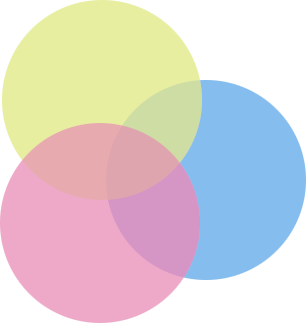
\includegraphics[width=3in]{images/logo.png}
\end{center}

\vfill
\begin{warning}
  This is a pre-release draft and has not yet been verified for accuracy.
  If you find any errors or have suggestions for improvement, please post
  an issue on the GitHub repository at
  \url{https://github.com/jlenthe/math-concepts-guide}.
\end{warning}
\begin{center}
    {\small This work is licensed under \textbf{CC BY-NC-SA 4.0}.\\
    To view a copy of this license, visit \url{https://creativecommons.org/licenses/by-nc-sa/4.0/}.}
\end{center}

\newpage
\tableofcontents
\newpage

\section*{Preamble}
We believe that mathematics is a powerful language that everyday people can
use to express and communicate ideas with far greater precision than can be
attained with natural language alone. This document provides a reference for
basic mathematical notation and definitions. It is intended to be accessible
to non-experts and to serve as a quick reference. Sets, relations, and
functions are covered in this document.

% Main content sections
\section{Sets}

\begin{definition}{Set}{set}
  A \textbf{set} is a collection of distinct objects.
\end{definition}
\begin{table}[H]
  \centering
  \begin{tabular}{p{1.5in} p{3in}}
    \toprule
    \textbf{Set} & \textbf{Description} \\
    \midrule
    \( A = \{ 1, 2, 3 \} \) & \( A \) is the set of numbers 1, 2, and 3. \\
    \( B = \{ x, y, z \} \) & \( B \) is the set of variables \(x\), \(y\), and \(z\). \\
    \( C = \{ \text{Apple}, \text{Orange} \} \) & \( C \) is the set of words Apple and Orange. \\
    \bottomrule
  \end{tabular}
  \caption{Basic Examples of Sets}
\end{table}

Sets have many practical uses. Often a set is used to specify a group from which
an object can be chosen, such as a restaurant menu or a product catalog. Sets can
group together related objects, such as the items on a sales receipt.
Sets can also be used to represent entire types of mathematical objects such as
numbers, lines, or polygons.

Some key points to know about sets include:
\begin{itemize}
  \item Sets may not have duplicate elements. So \( \{ 1, 1, 2 \} \) is not a set
     as such, but essentially just the set \( \{ 1, 2 \} \).
   This is what is meant when we say \emph{distinct objects}.
  \item Sets may contain objects of any type including numbers, strings, or other sets
   or contain objects of different types. So \( \{ 1, \text{Apple}, \{ 1, 2, 3\} \} \) is a valid set.
  \item Sets may have any number of elements including zero elements or be infinite.
  \item Sets are not inherently ordered. So \( \{ 1, 2, 3 \} \) is the same set as \( \{ 3, 2, 1 \} \).
   It is possible to impose an order on a set, but an ordering is separate from the set itself.
  \item A set cannot contain itself as an element. A statement such as \( A = \{ A \} \)
    is invalid since it creates a paradox.
\end{itemize}

\begin{definition}{Empty Set}{emptyset}
  The \textbf{empty set} or \textbf{null set} is the set that contains no elements
  and is denoted by \( \emptyset \) or \( \{ \} \).
\end{definition}

The empty set is an important and powerful concept. It gives us a precise way to say
things like ``there is no one on our team with a birthday in March'' or ``there are no
solutions to this equation''

\begin{definition}{Cardinality}{cardinality}
  The \textbf{cardinality} of a finite set is the number of elements in the set and is
  denoted by \( |A| \) where \( A \) is the set. The cardinality of the empty
  set is zero, \( |\emptyset| = 0 \). The cardinality of an infinite set is simply said
  to be infinite.
\end{definition}

Cardinality is useful because it allows us to quantify and compare the size of sets. It
gives us a precise way to express things like ``I bought 20 items at the grocery store
last week whereas this week I only bought 15 items''. And the concept of cardinality
fully applies to sets that are unbounded or infinite in size as well.

\begin{table}[H]
  \centering
  \begin{tabular}{p{2in} p{1in} p{2in}}
    \toprule
    \textbf{Set} & \textbf{Cardinality} & \textbf{Description} \\
    \midrule
    \( A = \{ 1, 2, 3 \} \) & \( |A| = 3 \) & The cardinality of set \(A\) is 3. \\
    \( B = \{ w. x, y, z \} \) & \( |B| = 4 \) & The cardinality of set \(B\) is 4. \\
    \( C = \{ \text{Apple}, \text{Orange} \} \) & \( |C| = 2 \) & The cardinality of set \(C\) is 2. \\
    \( D = \{ 1, 2, 3, 4, 5, 6, 7, 8, 9, 10 \} \) & \( |D| = 10 \) & The cardinality of set \(D\) is 10. \\
    \( E \) is the set of all even integers & \( |E| \) is infinite & The cardinality of set \(E\) is infinite. \\
    \( F = \{ \{1, 2, 3\}, \{4\}, \emptyset \} \) & \( |F| = 3 \) & Set \(F\) contains three elements, each of which is itself a set. \\
    \bottomrule
  \end{tabular}
  \caption{Examples of Set Cardinality}
\end{table}

\begin{advancedTopic}
  Infinite sets do not all have the same cardinality—there are different infinite cardinalities
  that can be distinguished. For simplicity here, though, we just refer to infinite sets. For more
  information, look up the topic of \emph{transfinite cardinals}.
\end{advancedTopic}

Sets of numbers, such as the real numbers and integers, are commonly referenced and are
designated with special symbols as shown in the follow table. These number sets are defined in section
\ref{sec:numbers}.
\begin{table}[H]
  \centering
  \begin{tabular}{p{1in} p{2in}}
  \toprule
  \textbf{Set Name} & \textbf{Description} \\
  \midrule
  \(\mathbb{N}\) & Natural numbers \\
  \(\mathbb{Z}\) & Integers \\
  \(\mathbb{Q}\) & Rational numbers \\
  \(\mathbb{R}\) & Real numbers \\
  \(\mathbb{C}\) & Complex numbers \\
  \bottomrule
  \end{tabular}
  \caption{Symbols for Common Sets of Numbers}
\end{table}

\begin{definition}{Set Membership}{membership}
  The symbol \( \in \) is used to assert that an element is a member of a set.
  The symbol \( \notin \) is used to assert that an element is not a member of a set.
\end{definition}

\begin{table}[H]
  \centering
  \begin{tabular}{p{1.5in} p{2in}}
    \toprule
    \textbf{Set} & \textbf{Examples of True Assertions} \\
    \midrule
    \( A = \{ 1, 2, 3 \} \) & \( 1 \in A \), \( 4 \notin A \) \\
    \( B = \{ x, y, z \} \) & \( x \in B \), \( a \notin B \) \\
    \( C = \{ \text{Apple}, \text{Orange} \} \) & \( \text{Apple} \in C \), \( \text{Banana} \notin C \) \\
    \( D = \emptyset \) & \( 0 \notin D \), \( x \notin D \) for all \(x \in \mathbb{R} \) \\
    \( E = \{ 2, 4, 6, 8 \} \) & \( 4 \in E \), \( 5 \notin E \) \\
    \( F = \{ \{1, 2\}, \{3\}, \emptyset \} \) & \( \{1, 2\} \in F \), \( \emptyset \in F \), \( 2 \notin F \) \\
    \bottomrule
  \end{tabular}
  \caption{Set Membership Examples}
\end{table}

\begin{definition}{Set Builder Notation}{set-builder-notation}
  Sets expressed or defined by \textbf{set builder notation} are sets that are defined by
  the properties of their elements with the following form:
  \[
    A = \{ x \in S \mid P(x) \}
  \]
  where \( S \) is a set and \( P(x) \) is a property that must hold true for \( x \) to be
  an element of \( A \). The vertical bar \( | \) is typically read as ``such that''.
\end{definition}

Set builder notation gives us a powerful way to define sets. With set builder notation, we can
define sets using the properties that all members of the set must satisfy. This eliminates the
need to enumerate all the elements of the set exhaustively. Defining a set with set builder
can result in a set that is finite or infinite in cardinality.

\begin{table}[H]
  \centering
  \begin{tabular}{p{2in} p{3in}}
    \toprule
    \textbf{Set} & \textbf{Description} \\
    \midrule
    \( \{ x \in \mathbb{N} \mid x < 5 \} \) & The set of all natural numbers less than 5. \\
    \( \{ x \in \mathbb{Z} \mid x^2 < 10 \} \) & The set of all integers whose square is less than 10. \\
    \( \{ x \in \mathbb{Z} \mid x \text{ is even} \} \) & The set of all integers that are even. \\
    \( \{ x \in \mathbb{R} \mid x^2 - 25 = 0\} \) & The set of all real numbers whose square minus 25 equals zero.\\
    \( \{ x \in \mathbb{R} \mid x > 0, x < 0\} = \emptyset \) &
      The set of all real numbers both greater than zero and less than zero, i.e. the empty set.  \\
    \end{tabular}
  \caption{Set Builder Notation Examples}
\end{table}

\begin{definition}{Extended Set Builder Notation}{extended-set-builder-notation}
  The \textbf{extended set builder notation} is a more general form of set builder notation
  that allows for more complex expressions to the left of the vertical bar \( | \).
  It takes the form:
  \[
    A = \{ E \mid P_1, P_2, ... \}
  \]

  where \( E \) is an expression involving one or more variables and \( P_1, P_2, ... \) are
  one or more properties involving those variables that all must hold true for \( E \) to be an
  element of \( A \).
\end{definition}

The extended set builder notation gives us a bit more flexibility in defining sets. It allows us
to define the members of a set by modifying members of another set and subject to one
or more properties.

\begin{table}[H]
  \centering
  \begin{tabular}{p{2in} p{3in}}
    \toprule
    \textbf{Set} & \textbf{Description} \\
    \midrule
    \( \{ 2^n \mid n \in \mathbb{Z} \} \) & The set of all integer powers of 2. \\
    \( \{ n^2 \mid n \in \mathbb{Z}, n > 0 \} \) & The set of all positive perfect squares. \\
    \( \{ x^3 \mid x \in \mathbb{R}, 5 \le x \le 10 \} \) &
      The set of cubes of all real numbers between 5 and 10. \\
    \bottomrule
  \end{tabular}
  \caption{Extended Set Builder Notation Examples}
\end{table}

\begin{definition}{Set Equality}{setEquality}
  Two sets \( A \) and \( B \) are equal, denoted by \( A = B \), if and only if
  every element of \( A \) is also an element of \( B \) and every element of \( B \)
  is also an element of \( A \). Sets that are not equal are denoted by \( A \neq B \).
\end{definition}

Having a precise definition of set equality allows us to describe two sets in different
ways and determine if they are equal or not.

\begin{table}[H]
  \centering
  \begin{tabular}{p{2in} p{0.75in} p{2.25in}}
    \toprule
    \textbf{Sets} & \textbf{Equality \newline Assertion} & \textbf{Description} \\
    \midrule
    \( A = \{ 1, 2, 3 \}, B = \{ 3, 2, 1 \} \) & \( A = B \) & Both sets contain exactly the same elements, order does not matter. \\
    \( A = \{ 1, 2, 3 \},\ B = \{ 1, 2, 3, 4 \} \) & \( A \neq B \) & \( B \) contains an extra element (4) not in \( A \). \\
    \( A = \emptyset,\ B = \{ \} \) & \( A = B \) & Both sets are empty, so they are equal. \\
    \( A = \{ 1, 2, 3 \},\ B = \{ 1, 2, \{3\} \} \) & \( A \neq B \) &
      \( B \) contains the set \( \{3\} \) as an element, not the number \( 3 \); thus, the sets are not equal. \\
    \( A = \{ x^2 \mid x \in \{ 2, 3 \} \},\ B = \{ 4, 9 \} \) & \( A = B \) & Both sets contain the same elements: squaring each
      element of \( \{2, 3\} \) gives \( 4 \) and \( 9 \), so \( A = \{4, 9\} = B \). \\
    \bottomrule
  \end{tabular}
  \caption{Examples of Set Equality}
\end{table}

\section{Tuples}
\begin{definition}{Tuple}{tuple}
  A \textbf{tuple} is a finite ordered list of elements.
\end{definition}

The word "tuple" is commonly pronounced as either “tuh-ple” or “too-ple”.

Tuples have many applications. Tuples can represent the coordinates of a point in space,
the state of a system, or the configuration of a machine. Tuples are also the building
blocks of other basic mathematical concepts such as relations and functions.

A tuple is often denoted using indexed elements, such as:
\[
  A = (a_1, \ldots, a_n)
\]
where each \( a_i \) is an element of the tuple, indexed by its position.

\begin{table}[H]
  \centering
  \begin{tabular}{ll}
    \toprule
    \textbf{Tuple} & \textbf{Description} \\
    \midrule
    \( A = (1, 2, 3) \) & Tuple with elements \( A_1 = 1 \), \( A_2 = 2 \), and \( A_3 =3 \) \\
    \( B = (x, y, z) \) & Tuple with elements \( B_1 = x \), \( B_2 = y \), and \( B_3 = z \) \\
    \( C = (\text{Apple}, \text{Orange}) \) & Tuple with elements \( C_1 = \text{Apple} \), \( C_2 = \text{Orange} \) \\
    \( D = (7, \{1, 2\}, (a, b)) \) & Tuple with elements \( D_1 = 7 \), \( D_2 = \{1, 2\} \), and \( D_3 = (a, b) \) \\
    \bottomrule
  \end{tabular}
  \caption{Tuple Examples}
\end{table}

Some key points to know about tuples include:
\begin{itemize}
  \item A tuple may have repeated elements. There is no requirement that the elements be distinct.
  \item A tuple may have zero elements.
  \item The number of elements in a tuple is called the \textbf{length} of the tuple.
  \item A tuple may contain objects of any type including numbers, strings, sets, or other tuples
   and elements of different types are allowed in the same tuple.
\end{itemize}

Tuples of specific lengths may have special names. The following table lists the names of tuples
of common lengths. Aside from \emph{ordered pair}, the names are not universally accepted and may
vary by author or context. So it is often best to simply use 4-tuple, 5-tuple, etc. to avoid
confusion.

\begin{table}[H]
  \centering
  \begin{tabular}{ll}
  \toprule
  \textbf{Tuple Length} & \textbf{Names} \\
  \midrule
  0 & empty tuple \\
  1 & singleton, single \\
  2 & ordered pair, pair \\
  3 & triple, triplet \\
  4 & quadruple \\
  5 & quintuple \\
  6 & sextuple \\
  7 & septuple \\
  8 & octuple \\
  \( n  \) & n-tuple \\
  \bottomrule
  \end{tabular}
  \caption{Names for Common Tuples}
\end{table}

\begin{advancedTopic}
  The concept of tuples has been extended to infinite length. For more
  information, look up the topic of \emph{Hilbert spaces}.
\end{advancedTopic}

\begin{definition}{Tuple Equality}{tupleEquality}
  Two tuples \( A \) and \( B \) are equal if and only if they have the same length and
  their corresponding elements are equal.
\end{definition}

The following table contains examples of comparison of tuples for equality.

\begin{table}[H]
  \centering
  \begin{tabular}{ll}
    \toprule
    \textbf{Tuples} & \textbf{Equality Assertion} \\
    \midrule
    \( A = (1, 2, 3),\ B = (1, 2, 3) \) & \( A = B \) \\
    \( A = (1, 2, 3),\ B = (3, 2, 1) \) & \( A \neq B \) \\
    \( A = (x, y, z),\ B = (x, y, z) \) & \( A = B \) \\
    \( A = (\text{Apple}, \text{Orange}),\ B = (\text{Orange}, \text{Apple}) \) & \( A \neq B \) \\
    \( A = (1, 2, 3),\ B = (1, 2) \) & \( A \neq B \) \\
    \( A = (\{1, 2\}, \{3\}),\ B = (\{1, 2\}, \{3\}) \) & \( A = B \) \\
    \( A = (1, \emptyset, \{2\}),\ B = (1, \{\,\}, \{2, 3\}) \) & \( A \neq B \) \\
    \bottomrule
  \end{tabular}
  \caption{Tuple Equality Examples}
\end{table}

\section{Set Inclusion}
Subsets and supersets describe the relationship between sets when one set is contained in
another set.

\begin{definition}{Subset}{subset}
  A set \( A \) is a \textbf{subset} of a set \( B \) if every element of
  \( A \) is also an element of \( B \).  This is denoted by \( A \subseteq B \).
\end{definition}

\begin{definition}
    {Superset}{superset}
    A set \( A \) is a \textbf{superset} of a set \( B \) if every element of
    \( B \) is also an element of \( A \). This is denoted by \( A \supseteq B \).
\end{definition}

Key notes about subsets and supersets:
\begin{itemize}
  \item Every set is a subset of itself, \( A \subseteq A \).
  \item Every set is a superset of itself, \( A \supseteq A \).
  \item The empty set is a subset of every set, \( \emptyset \subseteq A \).
  \item Every set is a superset of the empty set, \( A \supseteq \emptyset \).
\end{itemize}


\begin{definition}{Proper Subset}{properSubset}
  A set \( A \) is a \textbf{proper subset} of a set \( B \) if every element of
  \( A \) is also an element of \( B \) and \( A \neq B \). This is denoted by
  \( A \subset B \).
\end{definition}

\begin{definition}
    {Proper Superset}{properSuperset}
    A set \( A \) is a \textbf{proper superset} of a set \( B \) if every element of
    \( B \) is also an element of \( A \) and \( A \neq B \). This is denoted by
    \( A \supset B \).
\end{definition}

When we intuitively think of subsets and supersets, we think of one set being
contained in another set. That intuition corresponds to the concept of \emph{proper}
subsets and \emph{proper} supersets, since formally a set is a subset and
superset of itself.

\begin{definition}{Power Set}{powerSet}
  The \textbf{power set} of a set \( A \) is the set of all possible subsets of \( A \).
  This is denoted by \( \mathcal{P}(A) \).
\end{definition}

Power set examples:
\begin{itemize}
  \item \( A = \{ 1, 2 \} \), then \( \mathcal{P}(A) = \{ \emptyset, \{ 1 \}, \{ 2 \}, \{ 1, 2 \} \} \).
  \item \( B = \{ x, y, z \} \), then \( \mathcal{P}(A) = \{ \emptyset, \{ x \}, \{ y \}, \{ z \},
  \{ x, y \}, \{ x, z \}, \{ y, z \}, \{ x, y, z \} \} \).
  \item \( C = \{ \text{Apple}, \text{Orange} \} \), then \( \mathcal{P}(A) = \{ \emptyset,
  \{ \text{Apple} \}, \{ \text{Orange} \}, \{ \text{Apple}, \text{Orange} \} \} \).
  \item \( D = \{ 1, 2, 3 \} \), then \( \mathcal{P}(A) = \{ \emptyset, \{ 1 \}, \{ 2 \},
  \{ 3 \}, \{ 1, 2 \}, \{ 1, 3 \}, \{ 2, 3 \}, \{ 1, 2, 3 \} \} \).
\end{itemize}

\section{Set Operations}

Set operations are ways that two sets can be combined into a new set. The
foundational set operations are union, intersection, and difference. Union
combines all the elements from both sets. Intersection results in only the
elements common to both sets. And difference takes the elements of one
set away from another set.

\begin{definition}{Union}{union}
  The \textbf{union} of two sets \( A \) and \( B \) is the set of all elements
  that are in either \( A \) or \( B \) or both. This is denoted by \( A \cup B \).
\end{definition}

Union examples:
\begin{itemize}
  \item \( A = \{ 1, 2, 3 \} \) and \( B = \{ 3, 4, 5 \} \), then \( A \cup B = \{ 1, 2, 3, 4, 5 \} \).
  \item \( A = \{ x, y, z \} \) and \( B = \{ a, b, c \} \), then \( A \cup B = \{ x, y, z, a, b, c \} \).
  \item \( A = \{ \text{Apple}, \text{Orange} \} \) and \( B = \{ \text{Banana}, \text{Grape} \} \), then
  \( A \cup B = \{ \text{Apple}, \text{Orange}, \text{Banana}, \text{Grape} \} \).
  \item \( A = \{ x \in \mathbb{R} \mid x < -10 \} \) and \( B = \{ x \in \mathbb{R} \mid x > 10 \} \), then
  \( A \cup B = \{ x \in \mathbb{R} \mid x < -10 \text{ or } x > 10 \} \).
\end{itemize}

\begin{definition}{Intersection}{intersection}
  The \textbf{intersection} of two sets \( A \) and \( B \) is the set of all
  elements that are in both \( A \) and \( B \). This is denoted by \( A \cap B \).
\end{definition}

Intersection examples:
\begin{itemize}
  \item \( A = \{ 1, 2, 3 \} \) and \( B = \{ 3, 4, 5 \} \), then \( A \cap B = \{ 3 \} \).
  \item \( A = \{ x, y, z \} \) and \( B = \{ a, b, c \} \), then \( A \cap B = \emptyset \).
  \item \( A = \{ \text{Apple}, \text{Orange} \} \) and \( B = \{ \text{Banana}, \text{Orange}, \text{Grape} \} \), then
  \( A \cap B = \{ \text{Orange} \} \).
  \item \( A = \{ x \in \mathbb{R} \mid x < 10 \} \) and \( B = \{ x \in \mathbb{R} \mid x > 5 \} \), then
  \( A \cap B = \{ x \in \mathbb{R} \mid 5 < x < 10 \} \).
\end{itemize}

\begin{definition}{Difference}{difference}
  The \textbf{difference} of two sets \( A \) and \( B \) is the set of all
  elements that are in \( A \) but not in \( B \). This is denoted by \( A - B \).
\end{definition}

The following table shows the definition of the set operations using set builder notation.
\begin{table}[H]
  \centering
  \begin{tabular}{p{1in} p{3in}}
    \toprule
    \textbf{Set Operation} & \textbf{Definition in Set Builder Notation} \\
    \midrule
    Union & \( A \cup B = \{ x \mid x \in A \text{ or } x \in B \} \) \\
    Intersection & \( A \cap B = \{ x \mid x \in A \text{ and } x \in B \} \) \\
    Difference & \( A - B = \{ x \mid x \in A \text{ and } x \notin B \} \) \\
    \bottomrule
  \end{tabular}
  \caption{Set Operations in Set Builder Notation}
\end{table}

\begin{definition}{Cartesian Product}{cartesianProduct}
  The \textbf{Cartesian product} of two sets \( A \) and \( B \) is the set of all
  ordered pairs \( (a, b) \) where \( a \in A \) and \( b \in B \). This is denoted by
  \( A \times B \).
  \medskip
  When a set is taken in a Cartesian product with itself, exponential notation is used:
  \begin{align*}
    A^2 &= A \times A \\
    A^3 &= A \times A \times A \\
    &\vdots \\
    A^n &= A \times A \times \ldots \times A
  \end{align*}
\end{definition}
Cartesian product examples:
\begin{itemize}
  \item \( A = \{ 1, 2 \} \) and \( B = \{ 3, 4 \} \), then
    \( A \times B = \{ (1, 3), (1, 4), (2, 3), (2, 4) \} \).
  \item \( C = \{ x, y \} \) and \( D = \{ a, b, c \} \),
    then \( C \times D = \{ (x, a), (x, b), (x, c), (y, a), (y, b), (y, c) \} \).
  \item \( E = \{ \text{Apple}, \text{Orange} \} \)
     and \( F = \{ 1, 2 \} \), then \\
     \( E \times F = \{ (\text{Apple}, 1), (\text{Apple}, 2), (\text{Orange}, 1), (\text{Orange}, 2) \} \).
  \item \( G = \{ 1, 2 \} \) and \( H = \{ x, y, z \} \), then \( G \times H = \{ (1, x), (1, y), (1, z), (2, x), (2, y), (2, z) \} \).
\end{itemize}

Looking at a common Cartesian product, \( \mathbb{R}^2 \), we can precisely describe it
as
\[
  \mathbb{R}^2 = \mathbb{R} \times \mathbb{R} = \{ (x, y) \mid x, y \in \mathbb{R} \}
\].

\section{Relations}
Relations are used to describe how elements of various sets
are related to each other. For example, comparisons of numbers such as
\( a < b \) can be defined as relations.

\begin{definition}{Relation}{relation}
  A \textbf{relation} on sets \( A \) and \( B \) is any subset of the
  Cartesian product \( A \times B \).
\end{definition}

Relation examples:
\begin{itemize}
  \item The less-than relation on \( \mathbb{R} \) may be defined as:
    \[
      \{ (x, y) \in \mathbb{R} \times \mathbb{R} \mid x < y \}
    \]
  \item The integer-squared relation on \( \mathbb{Z} \) may be defined as:
    \[
      \{ (x, y) \in \mathbb{Z} \times \mathbb{Z} \mid y = x^2 \}
    \]
  \item The natural square-root relation is a relation from \( \mathbb{N} \) to \( \mathbb{R} \)
  (i.e. a subset of \( \mathbb{N} \times \mathbb{R} \)) and may be defined as:
    \[
      \{ (x, y) \in \mathbb{N} \times \mathbb{R} \mid y = +\sqrt{x} \}
    \]
\end{itemize}

Relations often have special properties that are useful to identify.

\begin{definition}{Reflexive}{reflexive}
  A relation \( R \) on set \( A \) is \textbf{reflexive} if for all \( a \in A \), \( (a, a) \in R \).
\end{definition}

\begin{definition}{Irreflexive}{irreflexive}
  A relation \( R \) on set \( A \) is \textbf{irreflexive} if for all \( a \in A \), \( (a, a) \notin R \).
\end{definition}

A reflexive relation is one where every element is related to itself. An irreflexive relation is one where
no element is related to itself. A relation that is neither reflexive nor irreflexive has some elements
that are related to themselves and some that are not.

\begin{definition}{Symmetric}{symmetric}
  A relation \( R \) on set \( A \) is \textbf{symmetric} if for all \( a, b \in A \), if \( (a, b) \in R \) then
  \( (b, a) \in R \).
\end{definition}

A symmetric relation is one where the relation has no sense of direction. It indicates that two elements are
intrinsically mutually related to each other in some way.

\begin{definition}{Transitive}{transitive}
  A relation \( R \) on set \( A \) is \textbf{transitive} if for all \( a, b, c \in A \), if \( (a, b) \in R \) and
  \( (b, c) \in R \) then \( (a, c) \in R \).
\end{definition}

A transitive relation implies some kind of overarching structure or relatability among all the elements
such as the ability to strictly order numbers in a consistent way.

\begin{definition}{Equivalence Relation}{equivalence-relation}
  A relation \( R \) is an \textbf{equivalence relation} if it is reflexive, symmetric, and transitive.
\end{definition}

An equivalence relation, as defined above, specifies the properties a relation must have to embody
the general concept of "equivalence", but it does not specify the full meaning of a particular
equivalence. Multiple equivalence relations can be defined on the same set with different meanings.
For example, on the set of natural numbers \( \mathbb{N} \), we can define equivalence relations based
on numeric quantity, parity (even or odd), or divisibility. All such relations would have the properties
of reflexivity, symmetry, and transitivity.

For example, we could define an equivalence relation on \( \mathbb{N} \) that corresponds
to normal numerical equality, but we could also define parity equality as an equivalence relation where two
natural numbers are "equivalent" if they are both even or both odd.

\begin{table}[H]
  \centering
  \begin{tabular}{p{2in} p{3in}}
  \toprule
  \textbf{Comparison Relation} & \textbf{Properties} \\
  \midrule
  \( < \) (less than) & transitive, irreflexive \\
  \( \leq \) (less than or equal to) & reflexive, transitive \\
  \( > \) (greater than) & transitive, irreflexive \\
  \( \geq \) (greater than or equal to) & reflexive, transitive \\
  \( = \) (equal) & reflexive, symmetric, transitive \\
  \( \neq \) (not equal) & irreflexive, symmetric \\
  \bottomrule
  \end{tabular}
  \caption{Properties of Number Comparisons}
\end{table}


\section{Functions}

Functions are a construct that maps elements from one set to another.

\begin{definition}{Function}{function}
  A \textbf{function} \( f \) from a set \( A \) to a set \( B \) is a relation 
  \( f \subseteq A \times B \) such that for every element \( a \) in \( A \), 
  there is exactly one element \( b \) in \( B \) with \( (a, b) \in f \). 
  The set \( A \) is called the \textbf{domain} of the function, and the set 
  \( B \) is called the \textbf{codomain}. The value \( f(a) = b \) is called the 
  \textbf{image} of \( a \), and is often read as “\( f \) of \( a \).”

  \medskip

  The set of all images of elements in \( A \) is called the \textbf{range} of 
  the function.

  \medskip

  The domain and codomain of a function \( f \) may be denoted by \( f: A \to B \).
\end{definition}

Some key notes about functions:
\begin{itemize}
  \item The range of a function is the set of all actual outputs and, by 
    definition, is a subset of the codomain.
  \item It is common for the domain and codomain to be the same set, but it is not 
    required.
  \item Specific functions may be defined by a formula, a set of properties that hold true, 
    or an algorithm.
\end{itemize}

Often functions are intuitively thought as a process mapping an \textbf{input} to 
an \textbf{output}. Using this terminology:
\begin{itemize}
  \item The input is an element of the domain.
  \item The output is an element of the codomain.
  \item The function is the process or method that maps the input to the output.
  \item The image is the output of the function.
  \item The range is the set of all possible outputs.
\end{itemize}

An example of a function defined by a formula is the function \( f: \mathbb{R} \to \mathbb{R} \) 
defined by:
\[
  f(x) = x^2
\]
\noindent This function takes a real number \( x \) as input and returns the square of \( x \) as 
output. 

An example of a function defined by its properties is the absolute value function 
\( f: \mathbb{R} \to \mathbb{R} \) defined as:
\[
  f(x) = \begin{cases}
    x & \text{if } x \geq 0 \\
    -x & \text{if } x < 0
  \end{cases}
\]
  
An example of a tabulated function is the function \( f: \mathbb{A} \to \mathbb{A} \) 
where \( A = \{ 0, 1, 2, 3 \}\) defined by:
\begin{table}[H]
  \centering
  \begin{tabular}{cc}
    \toprule
    \textbf{\(n\)} & \textbf{\(f(n)\)} \\
    \midrule
    0 & 1 \\
    1 & 2 \\
    2 & 3 \\
    3 & 0 \\
    \bottomrule
  \end{tabular}
  \caption{Tablulated Function Example}
\end{table}
\noindent This function adds 1 to the input and wraps around to 0 when the input is 3.

Functions may also take tuples as input. Typically the domain set is written as a Cartesian 
product. For example, the function \( f: \mathbb{R}^2 \to \mathbb{R} \) defined by:
\[
  f(x, y) = x^2 + y^2
\]
\noindent This function takes a pair of real numbers \( (x, y) \) as input and returns the sum of 
the squares of \( x \) and \( y \) as output. Similarly, with 3 inputs \( f: \mathbb{R}^3 \to 
\mathbb{R} \) defined by:
\[
  f(x, y, z) = x^2 + y^2 + z^2
\]


\section{Logic}

Mathematical logic gives us a way to express statements involving
strictly true and false values.

\begin{definition}{Propositional Variable}{propositionalVariable}
  A \textbf{propositional variable} is a variable with a value from the set
  \( \mathbb{B} = \{ \text{True}, \text{False} \} \). A propositional variable
  is sometimes called a Boolean variable.
\end{definition}

\begin{definition}{Proposition}{proposition}
  A \textbf{proposition} is a statement that is either true or false but not both.
\end{definition}

A proposition is so called because it may be a question to be answered,
a statement of truth or falsehood, or a claim to be proved or disproved
depending on the context.

Propositional variables may be combined to form more complex propositions with
logical operators. The most common and familiar logical operators are \textbf{and}, \textbf{or},
and \textbf{not}. These operators have special symbols as delineated in the
following table:
\begin{table}[H]
  \centering
  \begin{tabular}{cc}
    \toprule
    Logical Operator & Symbol \\
    \midrule
    and & \( \land \) \\
    or & \( \lor \) \\
    not & \( \lnot \) \\
    \bottomrule
  \end{tabular}
  \caption{Logical Operators and Symbols}
\end{table}

\begin{definition}{Logical Operator}{logicalOperator}
  A \textbf{logical operator} is a function \( f: \mathbb{B}^n \to \mathbb{B} \),
  for \( n \in \mathbb{N} \) and \( n \ge 1 \) that takes one or more propositional variables
  as input and returns a value in \( \mathbb{B} \).
\end{definition}

Usually logical operators take only 1 input (unary) or 2 inputs (binary). For such operators,
there are only 2 or 4 possible inputs, respectively, so typically such operators are
tabulated in a \emph{truth table}. The following truth tables define the "and", "or"
and "not" logical operators, respectively.
\begin{table}[H]
  \centering
  \begin{tabular}{cc}
    \toprule
   \(P\) & \( \lnot P \)  \\
    \midrule
    True & False \\
    False & True \\
    \bottomrule
  \end{tabular}
  \caption{Truth Table for "not"}
\end{table}

\begin{table}[H]
  \centering
  \begin{tabular}{ccc}
    \toprule
    \(P\) & \(Q\) & \( P \land Q \)  \\
    \midrule
    True & True & True \\
    True & False & False \\
    False & True & False \\
    False & False & False \\
    \bottomrule
  \end{tabular}
  \caption{Truth Table for "and"}
\end{table}

\begin{table}[H]
  \centering
  \begin{tabular}{ccc}
    \toprule
    \(P\) & \(Q\) & \( P \lor Q \)  \\
    \midrule
    True & True & True \\
    True & False & True \\
    False & True & True \\
    False & False & False \\
    \bottomrule
  \end{tabular}
  \caption{Truth Table for "or"}
\end{table}

\begin{advancedTopic}
  While "and" and "or" are by far the most common logical binary operators,
  there are 16 binary logical operators in total. Some of these are important
  in digital circuit design and construction. For more information, look up
  the NAND, NOR, XOR, and XNOR operators or digital logic gates.
\end{advancedTopic}

Another logical operator of utmost importance is the \textbf{implication} operator,
which is denoted by the symbol \( \implies \). The proposition \( P \implies Q \),
means that if \( P \) is true, \( Q \) must also be true. We can define this more precisely
with a truth table:
\begin{table}[H]
  \centering
  \begin{tabular}{ccc}
    \toprule
    \(P\) & \(Q\) & \( P \implies Q \)  \\
    \midrule
    True & True & True \\
    True & False & False \\
    False & True & True \\
    False & False & True \\
    \bottomrule
  \end{tabular}
  \caption{Truth Table for "implication"}
\end{table}

\begin{advancedTopic}
  The notion that "\( \text{False} \implies \text{True} \) is True" is quite
  counterintuitive. It seems at odds with the typical meaning of the word "implies" in
  natural language and philosophical argumentation. This has been the subject of
  much philosophical discussion. For more information, look up \emph{material
  implication paradox}.
\end{advancedTopic}

\section{Numbers}

\begin{definition}{Natural Numbers}{naturalNumbers}
  The \textbf{Natural Numbers} are a set of numbers used for counting a discrete
  quantity of objects. They are denoted by the symbol \(\mathbb{N}\).
  \[
    \mathbb{N} = \{0, 1, 2, 3, \ldots\}
  \]
\end{definition}

The Natural Numbers may also be expressed in recursive set builder notation as
\[
  \mathbb{N} = \{ 0 \} \cup \{ n + 1 \mid n \in \mathbb{N} \}
\]
In other words, we begin with 0 as a natural number, and then each subsequent number
is formed by adding 1 to a number already in the set. This reflects the idea of
natural numbers as the basic instrument of counting.

Note that some definitions of the natural numbers exclude zero, defining
\(\mathbb{N} = \{1, 2, 3, \ldots\}\). Here, we include zero as the smallest natural
number because we find it useful and intuitive to be able to quantify emptiness
or nothingness with a natural number.

\begin{definition}{Integers}{integers}
  The \textbf{Integers} are a set of numbers that include all the natural numbers
  and, in addition, their negatives.
  They are denoted by the symbol \(\mathbb{Z}\).
  \[
    \mathbb{Z} = \{\ldots, -3, -2, -1, 0, 1, 2, 3, \ldots\}
  \]
\end{definition}

The Integers may also be expressed in set builder notation by building on the Natural Numbers
and adding their negatives to the set:
\[
  \mathbb{Z} = \mathbb{N} \cup \{-n \mid n \in \mathbb{N}, n > 0\}
\]

\begin{definition}{Real Numbers}{realNumbers}
  The \textbf{Real Numbers}, denoted by \(\mathbb{R}\), are the set of values that can be placed
  on an infinite, continuous, ordered number line. They include all quantities that represent
  continuous magnitudes such as length, time, and mass—in contrast to discrete quantities like
  counts or whole numbers.
\end{definition}

This definition may seem a bit vague, so let's elaborate on it. An ordered number line is a
one-dimensional space that extends infinitely in both directions and any number can be
ordered relative to any other number. For example, if \( a \) and \( b \) are two real numbers,
then either \(a < b\), \(a = b\), or \(a > b\). A continuous number line means that there are
no gaps between the numbers. For example, between any two real numbers \( a \) and \( b \), there
exists another real number \( c \) such that \(a < c < b\).

\begin{definition}{Rational Numbers}{rationalNumbers}
  The \textbf{Rational Numbers} are the subset of real numbers that can be expressed as the
  ratio of two integers, where the denominator is not zero. They are denoted by
  the symbol \(\mathbb{Q}\).
  \[
    \mathbb{Q} = \left\{ \frac{a}{b} \,\middle|\, a, b \in \mathbb{Z},\ b \ne 0 \right\}
  \]
\end{definition}

Rational numbers are the ordinary decimals and fractions that we encounter in everyday life, and include
natural numbers and integers. Some examples include:
\begin{itemize}
\item \(\frac{1}{2}\)
\item \(0.5\)
\item \(-3\)
\item \(\frac{3}{1}\)
\item \(2.75\)
\item \(\frac{11}{4}\)
\item \(0.3333\ldots\)
\end{itemize}

Infinitely repeating decimals, such as \(0.3333\ldots\) and \(0.\overline{12345}\), are also rational
numbers since they can be expressed as the integer ratios \(\frac{1}{3}\) and \(\frac{12345}{99999}\),
respectively. If the decimal representation of a number never terminates or repeats, then it is
not a rational number.

\begin{advancedTopic}
  People are often surprised to learn that \( 0.999\ldots \) is equal to \( 1 \). The proof of this
  fact is easily understood and well worth reading.
\end{advancedTopic}

\begin{definition}{Irrational Numbers}{irrationalNumbers}
  The \textbf{Irrational Numbers} are the subset of numbers that cannot be expressed
  as the ratio of two integers. They are denoted by the symbol \(\mathbb{R} \setminus \mathbb{Q}\).
  \[
    \mathbb{R} \setminus \mathbb{Q} = \left\{ x \,\middle|\, x \in \mathbb{R},\ x \notin \mathbb{Q} \right\}
  \]
\end{definition}

Irrational numbers include numbers like \(\sqrt{2}\), \(\pi\), and \( e \), which have been proven to
have no representation as a ratio of integers. Irrational numbers may be defined conceptually. For
example, \(\pi\) is defined as the ratio of the circumference of a circle to its diameter. Irrational
numbers are often handled abstractly through concepts and logic, or approximated numerically by rational numbers.

\begin{advancedTopic}
  The existence and nature of irrational numbers opens up a wide range of questions to explore. How can we know
  whether a number defined conceptually is rational or irrational? How can we approximate a given irrational
  number? Are there any irrational number that cannot be approximated? Which are there more of—rational or
  irrational numbers?
\end{advancedTopic}


\end{document}